\documentclass[tikz,border=6pt]{standalone}
\usepackage{amsmath}
\usepackage[europeanresistors]{circuitikz}
\usepackage{xcolor}
\usetikzlibrary{arrows.meta,positioning,decorations.pathmorphing}

\definecolor{blockblue}{HTML}{4A90D9}
\definecolor{linegray}{HTML}{333333}

\begin{document}
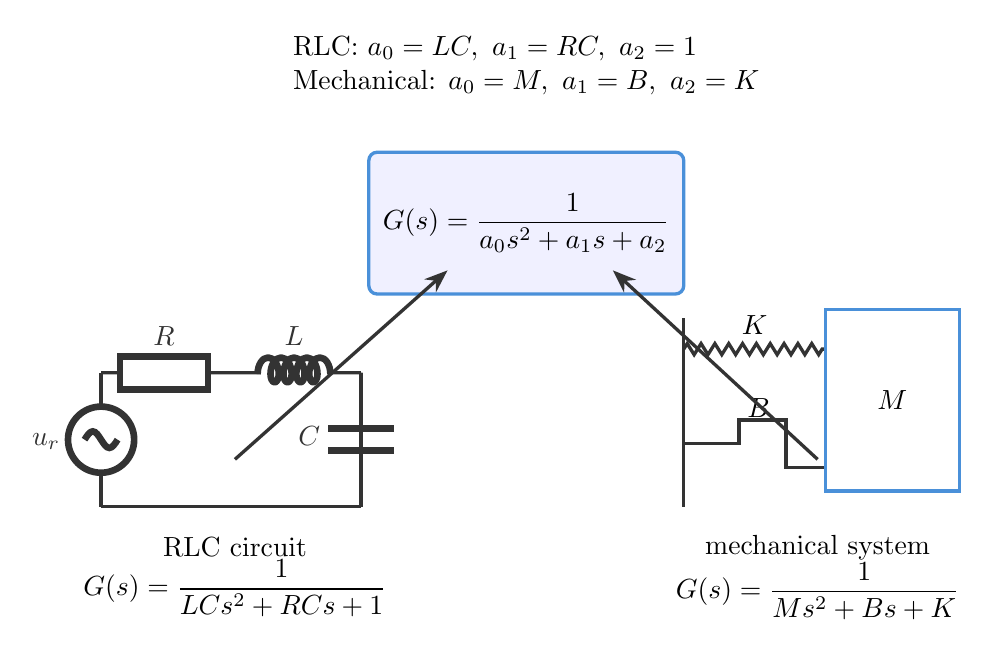
\begin{tikzpicture}[
  >=Stealth,
  line width=1.2pt,
  flow/.style={->, draw=linegray, line width=1.2pt},
  box/.style={draw=blockblue, rounded corners=3pt, minimum width=4.0cm, minimum height=1.8cm, align=center, fill=blue!6}
]
  \draw[linegray] (-6.2,0.1) to[R, l=$R$] (-4.6,0.1)
        to[L, l=$L$] (-2.9,0.1);
  \draw[linegray] (-2.9,0.1) -- (-2.9,-1.6);
  \draw[linegray] (-6.2,-1.6) -- (-2.9,-1.6);
  \draw[linegray] (-6.2,-1.6) to[sV, l=$u_r$] (-6.2,0.1);
  \draw[linegray] (-2.9,0.1) to[C, l_=$C$] (-2.9,-1.6);
  \node[align=center] at (-4.5,-2.5) {RLC circuit\\$G(s)=\dfrac{1}{LCs^2+RCs+1}$};

  \draw[linegray] (1.2,-1.6) -- (1.2,0.8);
  \draw[linegray, decorate, decoration={zigzag, segment length=5pt, amplitude=2pt}] (1.2,0.4) -- (3.0,0.4);
  \draw[linegray] (1.2,-0.8) -- (1.9,-0.8) -- (1.9,-0.5) -- (2.5,-0.5) -- (2.5,-1.1) -- (3.0,-1.1);
  \draw[fill=white, draw=blockblue] (3.0,-1.4) rectangle (4.7,0.9);
  \node at (3.85,-0.25) {$M$};
  \node at (2.1,0.7) {$K$};
  \node at (2.15,-0.35) {$B$};
  \node[align=center] at (2.9,-2.5) {mechanical system\\$G(s)=\dfrac{1}{Ms^2+Bs+K}$};

  \node[box] (common) at (-0.8,2.0) {$G(s)=\dfrac{1}{a_0s^2+a_1s+a_2}$};
  \draw[flow] (-4.5,-1.0) -- (-1.8,1.4);
  \draw[flow] (2.9,-1.0) -- (0.3,1.4);

  \node[align=left] at (-0.8,4.0) {
    RLC: $a_0=LC,\ a_1=RC,\ a_2=1$\\
    Mechanical: $a_0=M,\ a_1=B,\ a_2=K$
  };
\end{tikzpicture}
\end{document}
